\documentclass[10pt]{article}
\usepackage[a4paper,margin=16mm]{geometry}
\usepackage{mathptmx,graphicx,booktabs,hyperref}
\emergencystretch=2em
\setlength{\parindent}{0pt}\setlength{\parskip}{4pt}
\begin{document}
\begin{center}{\Large Uniform useful-yield experiment: preflight record}\\[5pt]
Quadratic-twist study, existing PR2381;25 October2026\end{center}

\textbf{No scientific run has started.} The protocol and compiled C++ producer
are prepared. A new repository launch gate requires S3 resume checkpoints;
existing user authorization excludes additional uploads, and no checkpoint-only
token is configured. This is an authorization/access hold, not a mathematical
obstruction or evidence against the hypothesis.

\section*{Stronger test, fixed before execution}
The completed F13 result has selected-target gains and matched losses. The
new protocol tests exact expected useful-rank gain, mean named solver degree
and rational collection-state recurrences under uniform independent nonidentity
queries. It covers all size-two/three bases on the already checked F43/F13
fixtures, both original/reduced S3 and every transported control. Source-DLP
maps and all prior proofs remain frozen. No new mean, recurrence, rank, solver
or scalar result is claimed by this preflight.

\begin{center}\begin{tabular}{lrr}\toprule
Deliverable & Planned & Executed scientific results\\\midrule
Base arms &96&0\\
Separate source targets &896&0\\
Uniform policy comparisons &210&0\\\bottomrule
\end{tabular}\end{center}
\begin{center}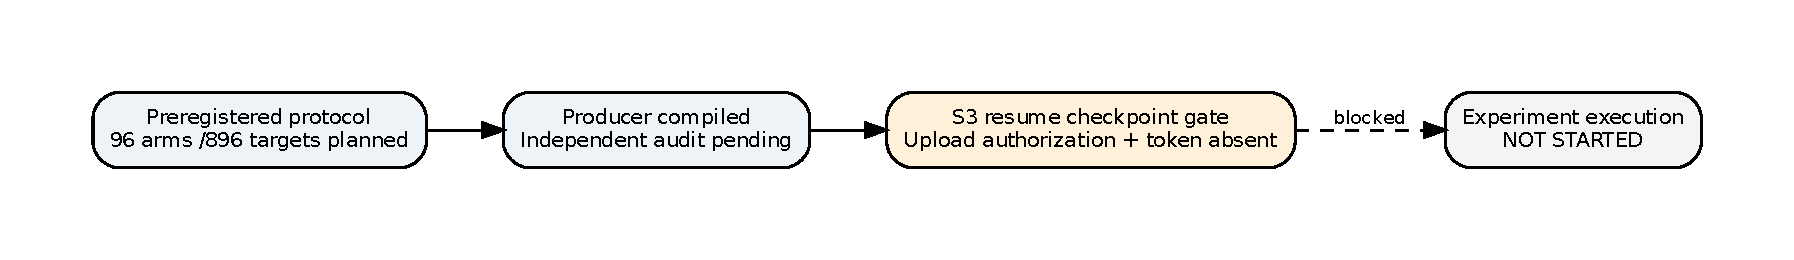
\includegraphics[width=\linewidth]{bridge.pdf}\end{center}
The producer compiles against existing GMP and OpenSSL. Earlier compile failures
from absent Boost headers and a missing functional include are preserved; no
producer execution followed them. Independent uniform Rust verification and
Lean recurrence proofs are still pending. The explicit F13 dual stays queued.
No timing, performance, regularity, hardness or complete-work claim is made.

\section*{New gate and reviewable authorization boundary}
Current main\path{20e8f44bba1f04e84a151e6f77e8fa752ebf7ad5} adds
``Resume checkpoints in S3 before every run''. Other runtimes must invoke the
gate before launching and must not launch if it fails. The official gate
invokes an upload after validating a complete resume note. A safe pre-init
check exits2 before uploading; a local resume note is now complete, so the
gate is not re-invoked without authorization. No skip flag or gate patch used.

The proposed scope is checkpoint-only writes in the existing
\texttt{setec-astronomy-artifacts} bucket under:
\begin{center}\small\ttfamily checkpoints/crypto/\\
codex\_\_quadratic-twist-evidence-import/\end{center}
Use the repository's
checkpoint-scoped token supplied through the environment. The first checkpoint can reference the published Git head and needs only its resume note, metadata,
archive and LATEST pointer. No previous credential or four-asset approval is
reused. Local checkpoint status, source hashes, compiled-source hashes and
exact resume contents are retained for review.

\section*{What can resume}
After explicit authorization and token configuration, use the unmodified gate,
finish/freeze the independent audit and faithful proof attempt, then execute the
bounded protocol with600-second native caps and a3600-second iteration budget.
All requested controls, exact results and a full result report remain required.
Until then only independent coding, repository review and ordinary validation
can proceed. The broader goal remains open; existing PR merge/CI/Conductor
holds are unchanged. No duplicate researcher or automation is created.
\end{document}
